%************************************************
\myChapter{Metoda}\label{ch:solution} % $\mathbb{ZNR}$
%************************************************

\section{Sprzęt}
\subsection{Opis}
W swojej pracy wykorzystałem sprzęt, który pokrótce omówię.\graffito{dodać schemat blokowy układu (post-it z monitora)}

\subsection{Elementy}
Sprzęt, abstrahując od dokładnego sposobu realizacji, składa się z dwóch markerów, których funkcje pełnią głośniki ultradźwiękowe, trzech odbiorników pod postacią mikrofonów ultradźwiękowych oraz mikrokontrolera \textsmaller{AVR Atmega8}. Dodatkowo w układzie zamontowanych jest 8 diod LED, które służą do nadzorowania stanu układu.

\subsection{Działanie}
\subsubsection{Po krótce}
Działanie mikrokontrolera sprowadza się do ciągłego, aktywnego prowadzenia pomiarów opóźnień czasów propagacji sygnału ultradźwiękowego pomiędzy markerami, a odbiornikami. Pozyskane w ten sposób dane przekazywane są za pomocą wyznaczonego protokołu do komputera, gdzie następuje ich dalsza obróbka.

Uproszczony schemat układu prezentuje rysunek~\ref{fig:device_scheme}.

\begin{figure}
 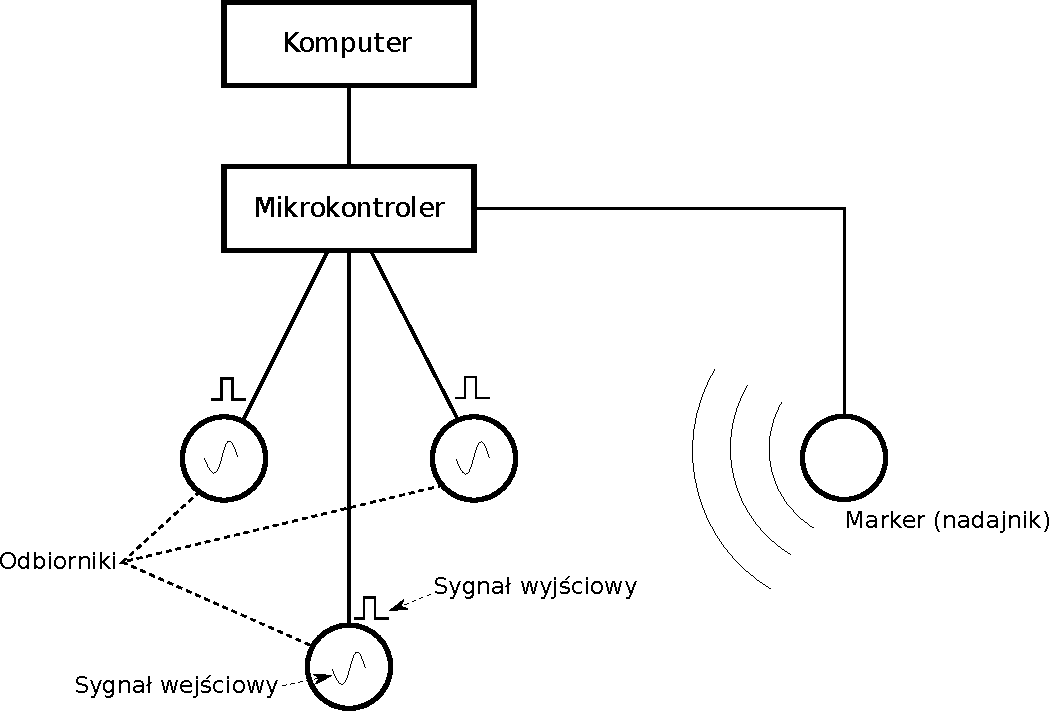
\includegraphics[width=\textwidth]{gfx/diagramy/schemat_blokowy_ukladu}
 \caption{Uproszczony schemat blokowy układu}
 \label{fig:device_scheme}
\end{figure}


\subsubsection{Po dłużce}
Działanie systemu opiera się o fakt, że dźwięk w powietrzu rozchodzi się ze stałą, znaną szybkością.

Ponieważ szybkość ta jest stała, można łatwo wyznaczyć odległość, jaką musiał przebyć dźwięk, aby dotrzeć do odbiornika:

\begin{equation}
 x = v \cdot t
 \label{eq:sound_distance}
\end{equation}
gdzie:\graffito{dodać informację nt. kalibracji - zmiana protokołu na obsługę potwierdzeń, oczekiwanie mikrokontrolera na potwierdzenie, rozpoczynanie kalibracją, wymóg piramidki do kalibracji}
\begin{description}
 \item[$x$] \ppauza~odległość przebyta przez dźwięk,
 \item[$v$] \ppauza~szybkość dźwięku w powietrzu,
 \item[$t$] \ppauza~czas od wysłania sygnału do jego dotarcia do odbiornika. 
\end{description}

Dane, jakie przekazywane są do komputera w celu dalszej obróbki zawierają, poza specyfikacją protokołu, tylko i wyłącznie odczyty z licznika dla każdego z odbiorników.

\paragraph{Przetwarzanie danych}
Aby dane były do czegoś użyteczne, wymagane jest ich przetworzenie. Przetwarzanie danych tej postaci może odbywać się różnorakimi metodami, np.:
\begin{itemize}
 \item rozpoznawanie gestów za pomocą sieci neuronowych,
 \item odtworzenie pozycji markera w trzech wymiarach,
 \item oczekiwanie na przemieszczenie markera do predefiniowanej pozycji,
 \item wiele innych.
\end{itemize}

\paragraph{Odtworzenie pozycji markera}
W celach demonstracyjnych postanowiłem pokazać, jak odtworzyć pozycję markera w trzech wymiarach korzystając tylko z informacji o względnym położeniu odbiorników oraz przekazywanych do komputera danych.
\newline
\newline
Ponieważ odbiorniki znajdują się w różnych, lecz znanych, położeniach w przestrzeni, odległość markera od każdego z nich może być różna.

Aby wyznaczyć położenie markera w trójwymiarowej przestrzeni, mając do dyspozycji odległości od każdego z odbiorników, należy założyć, że odbiorniki są środkami sfer, a promieniem każdej z nich \ppauza odległość, jaką przebył dźwięk od markera do tego odbiornika. Punkt przecięcia się tych sfer będzie pozycją markera.

\begin{figure}
  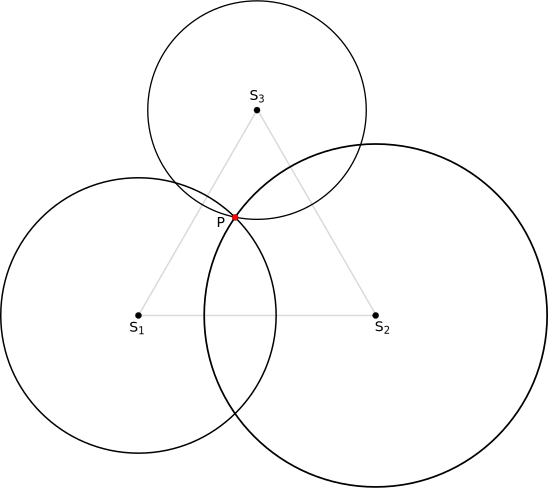
\includegraphics[width=\textwidth]{gfx/diagramy/schemat_przeciecia_sfer}
  \caption{Poglądowy schemat rozmieszczenia czujników}
  \label{fig:schema_spheres}
\end{figure}

Rysunek \ref{fig:schema_spheres}\graffito{W rysunku przyjęto widok ,,od przodu'', tzn. zachodzi $z = 0$ dla wszystkich elementów z wyjątkiem punktu $P$} prezentuje rozmieszczenie odbiorników na płycie testowej. Znajdują się one w punktach oznaczonych odpowiednio jako $S_1$, $S_2$ i $S_3$. Punkt $P$ to punkt przecięcia się sfer.

Ponieważ zastosowano tylko trzy odbiorniki, muszą one leżeć w jednej płaszczyźnie. Powoduje to, że będą istniały dokładnie dwa punkty przecięcia wspomnianych powyżej sfer \ppauza lustrzane do siebie względem płaszczyzny, w której znajdują się odbiorniki.\graffito{dodać notatkę w testach o możliwości wyeliminowania tego 'defektu' poprzez dodanie 4-tego odbiornika, niewspółpłaszczyznowego, jednak spowoduje to wzrost kosztów obliczeń}

Należy wziąć pod uwagę fakt, że zarówno marker jak i odbiorniki są urządzeniami ,,kierunkowymi'', umieszczonymi w tulejach, które powodują, że sygnał nie jest wysyłany dookólnie, lecz w pewnym \ppauza z grubsza określonym \ppauza kierunku, zaś amplituda sygnału odbieranego będzie większa, jeśli będzie on wpadał w tuleję, przez co szansa uznania go za poprawny jest znacznie większa.\graffito{sygnał dochodzący z boku może być ze słaby, aby został wyłapany}

Ta cecha układu została wykorzystana poprzez przeznaczenie układu do noszenia na tułowiu \ppauza łatwo zauważyć, że użytkownikowi ciężko byłoby przesunąć marker zbyt daleko do tyłu, gdyż ograniczałyby go stawy. 

Wykorzystując fakt, że człowiek trzyma ręce w większości przypadków przed sobą, szczególnie jeśli zamierza coś nimi robić, można spokojnie odrzucić jeden z punktów \ppauza ten który znajduje się ,,z tyłu''.

\paragraph{Trilateracja}
Metoda wyznaczenia trójwymiarowej pozycji znając odległości od trzech punktów o znanych współrzędnych nazywana jest \textit{trilateracją}\graffito{dodać info skąd to wiadomo}.

Problem wyznaczenia położenia markera można uprościć, przyjmując określony układ współrzędnych, w którym jeden z odbiorników znajduje się w początku ukłądu współrzędnych, jeden na osi $x$, a trzeci pozostaje ,,swobodny''\graffito{Współrzędna $z$ dla wszsytkich odbiorników równa jest~$0$}. Przyjmując takie rozmieszczenie, które zaprezentowane jest na rysunku \ref{fig:schema_coordinates}, odbiorniki mają współrzędne opdpowiednio:
\begin{matrix}
 $S_1$ & asd
\end{matrix}


\begin{figure}
  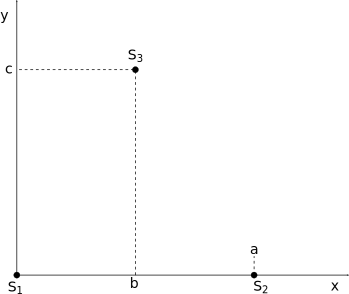
\includegraphics[width=\textwidth]{gfx/diagramy/schemat_uklad_wspolrzednych_clipped}
  \caption{Obrany układ współrzędnych}
  \label{fig:schema_coordinates}
\end{figure}


W celu pomiaru różnicy czasów zdecydowałem się wykorzystać ośmiobitowy timer/counter dostępny w używanym mikrokontrolerze.\graffito{to musi iść gdzieś indziej}

\section{Oprogramowanie}
\subsection{Wykresy}
W celach demonstracji działania stworzyłem program, który pokazuje dane odczytane z urządzenia w dwóch postaciach:
\begin{itemize}
 \item dane odczytane \ppauza rysowany jest wykres danych, jakie zostały wysłane przez urządzenie,
 \item dane przetworzone \ppauza rysowany jest wykres prezentujący pozycję wybranego markera w trzech wymiarach.
\end{itemize}
